\documentclass[]{article}
\usepackage{graphicx}
\graphicspath{{images/}}

%opening
\title{Random Projections}
\author{Felipe de A. Mello Pereira, Guilherme G. Schardong, \\ William Paulo Ducca Fernandes}

\begin{document}

\maketitle

\begin{abstract}

\end{abstract}

\section{Tables}

% latex table generated in R 3.2.3 by xtable 1.8-2 package
% Thu Sep 29 17:09:53 2016
\begin{table}[ht]
	\centering
	\begin{tabular}{rrrrrrrrr}
		\hline
		& 4 & 16 & 64 & 256 & 1024 & 4096 & 16384 & 65536 \\ 
		\hline
		gen\_proj\_mat\_ach & 0.01 & 0.04 & 0.17 & 0.67 & 2.69 & 10.74 & 42.99 & 715.77 \\ 
		gen\_proj\_mat\_gauss & 0.02 & 0.07 & 0.28 & 1.11 & 4.47 & 17.87 & 105.65 & 303.66 \\ 
		proj\_ach & 0.47 & 0.52 & 0.74 & 0.65 & 1.28 & 4.67 & 14.64 & 71.78 \\ 
		proj\_gauss & 0.47 & 0.52 & 0.74 & 0.59 & 1.19 & 4.90 & 16.18 & 79.58 \\ 
		proj\_pdist\_ach & 0.00 & 0.01 & 0.02 & 0.09 & 0.27 & 1.26 & 6.17 & 28.32 \\ 
		proj\_pdist\_gauss & 0.00 & 0.01 & 0.02 & 0.07 & 0.24 & 1.22 & 6.17 & 27.90 \\ 
		\hline
	\end{tabular}
\end{table}

% latex table generated in R 3.2.3 by xtable 1.8-2 package
% Thu Sep 29 17:10:18 2016
\begin{table}[ht]
	\centering
	\begin{tabular}{rrrrrrrrr}
		\hline
		& 4 & 16 & 64 & 256 & 1024 & 4096 & 16384 & 65536 \\ 
		\hline
		distortion\_ach & 6.35 & 2.22 & 0.94 & 0.48 & 0.23 & 0.10 & 0.05 & 0.03 \\ 
		distortion\_gauss & 5.92 & 2.58 & 1.14 & 0.46 & 0.22 & 0.10 & 0.06 & 0.03 \\ 
		p\_99\_error & 5.26 & 2.63 & 1.31 & 0.66 & 0.33 & 0.16 & 0.08 & 0.04 \\ 
		\hline
	\end{tabular}
\end{table}

\section{Plots}

\begin{figure}
	\centering
	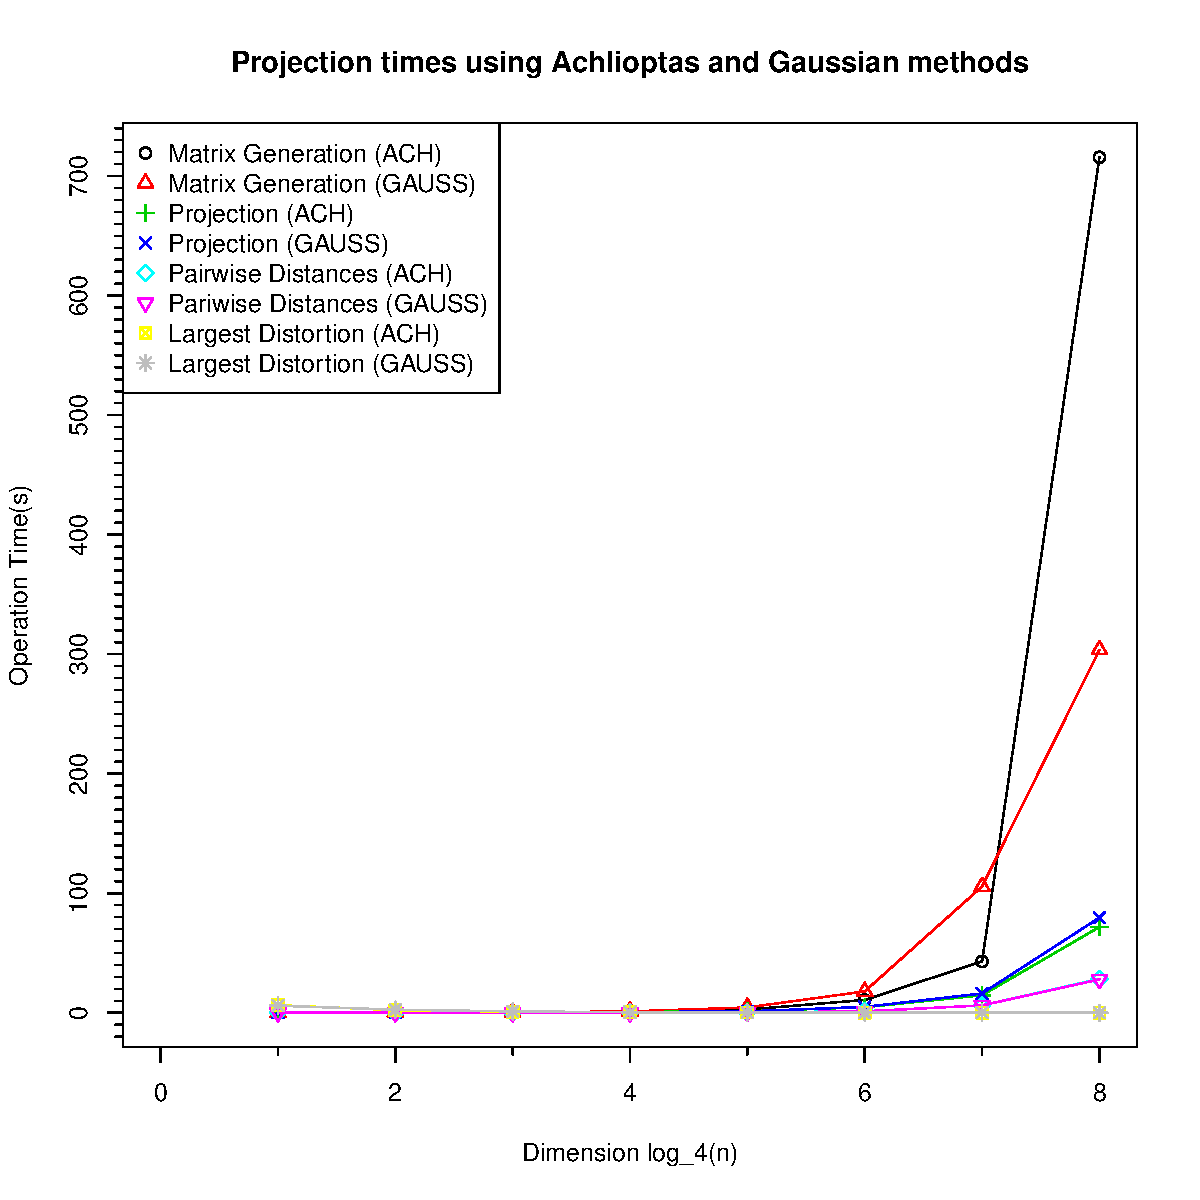
\includegraphics[width=\columnwidth]{projection-times_log-scale.pdf}
	\caption{}
\end{figure}

\begin{figure}
	\centering
	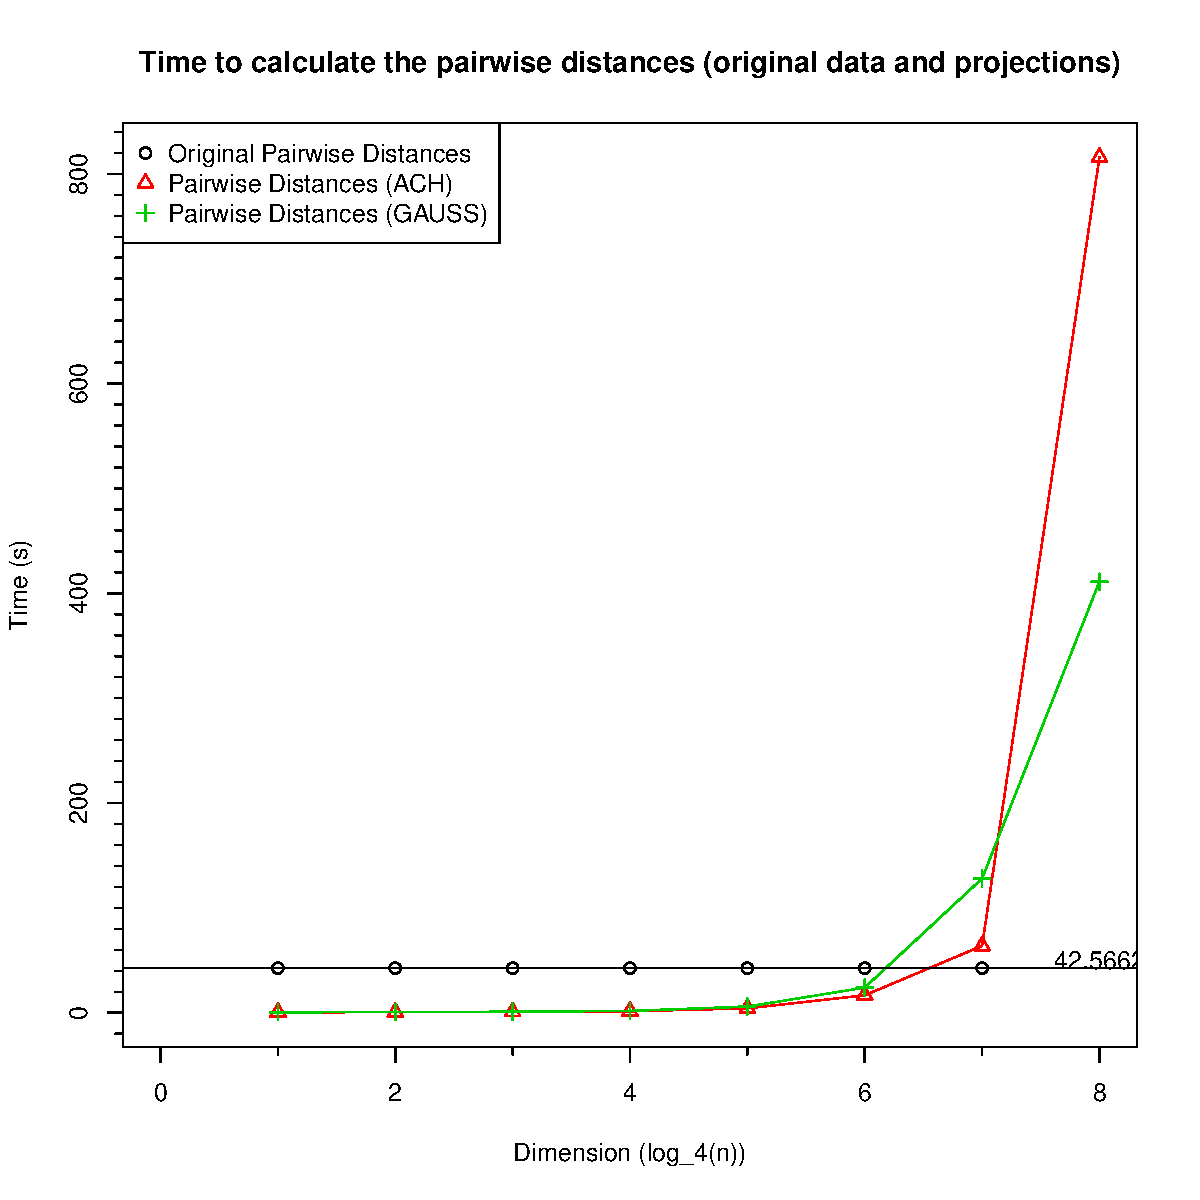
\includegraphics[width=\columnwidth]{proj-times-comparison.pdf}
	\caption{}
\end{figure}

\begin{figure}
	\centering
	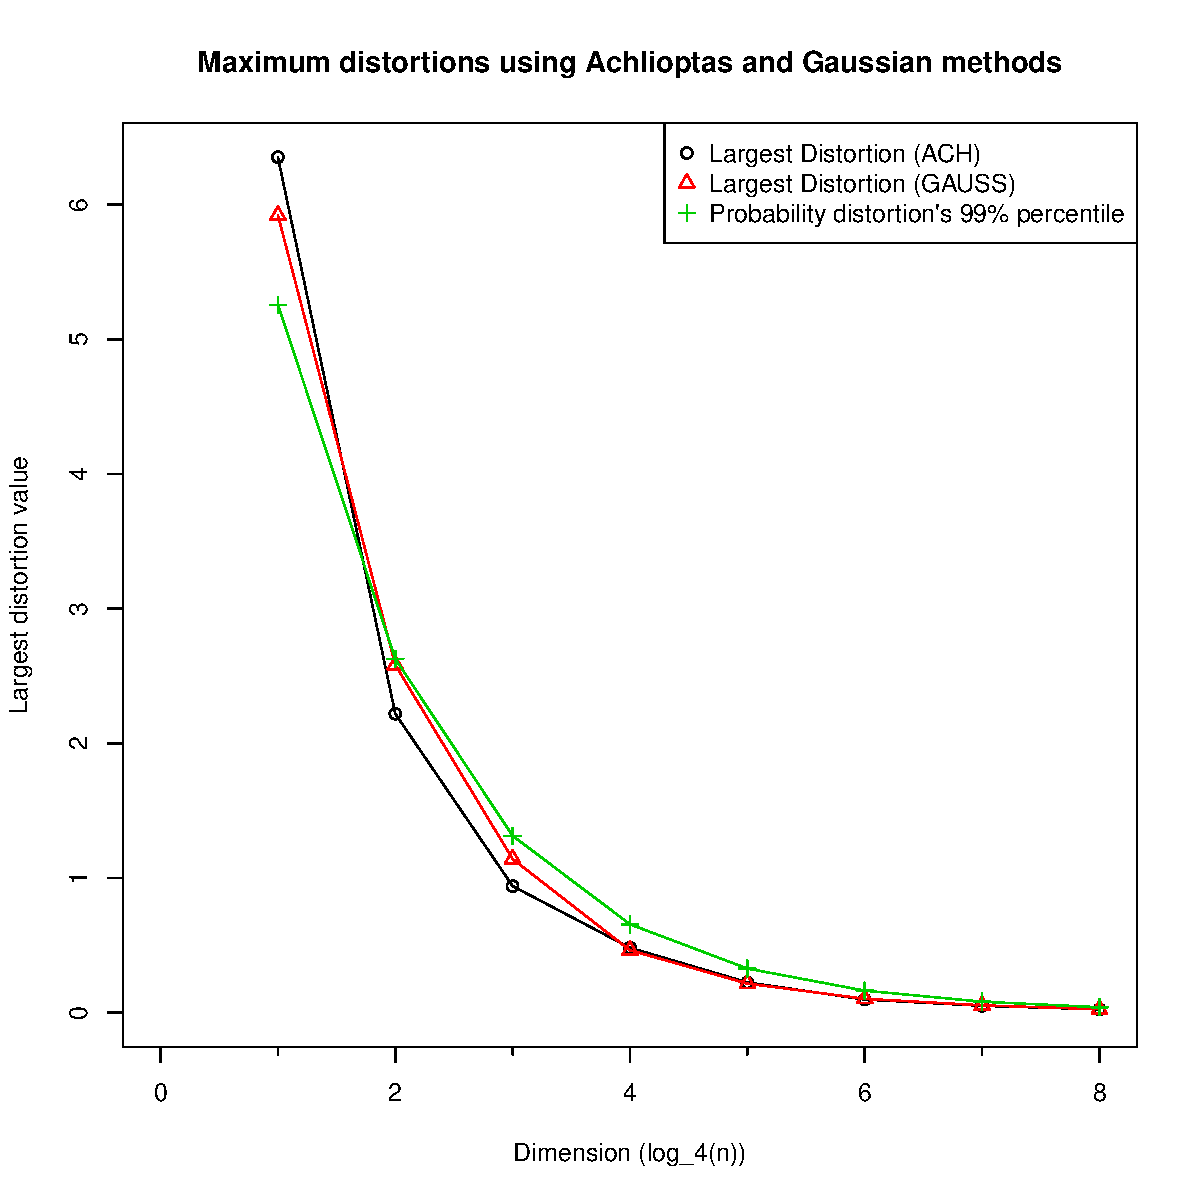
\includegraphics[width=\columnwidth]{maximum-distortions_log-scale.pdf}
	\caption{}
\end{figure}

\end{document}
